\section{Preliminaries}
add intro text here
<no need to discuss same level as greg's paper>
1. graph
    a. what does this mean?
    	i. nodes <what does this mean>
    	ii. edges <what does this mean>
    b. associated variables
    c. accounting for bus schedule
    d. group constraints
        a. meaning
    e. graph encodes connection bus-battery charger connection opportunities
    f. incidence matrix + linear algebra
    g. show picture of graph
2. Battery SOC
    a. Introduce new variables d_{i,j} g_{i,j}
    b. charging
        i. variable rate
	ii. variable rate adds edges to the graph (contribution)
	iii. show picture with d_{i,j} illustrated
    c. discharging
        i. delta is all that matters
	ii. comes from sim/real data (contribution)
3. Rate schedule
    a. consumption
    b. power, average power, demand charge (abstract)
        i. peak vs facilities demand charge
	ii. constraints for this
4. Fleet Operations
    a. Depot for night time charging
        i. one charger per bus
	ii. slow chargers
	iii. single rate charging
    b. Station for daytime charging
        i. limited number of chargers
	ii. fast/variable rate
    c. multiple graphs
        i. interconnections through SOC variables
	ii. show picture for this
5. Objective Function
6. Gurobi
7. Results
8. Future Work

\input{preliminaries/Graph.tex}
\subsection{Mixed Integer Linear Programs} 
insert text here

\section{Battery State of Charge}
The state of charge (SOC) is influenced in three ways; initial conditions, discharge events, and traversing charge nodes (as shown in figure \ref{fig:edgeTypes}).  There are SOC variables for each node representing an available bus, where the SOC value for the ith bus at SOC index j is denoted as $d_{i,j}$ as shown in figure \ref{fig:socDiagram}.  Note, there only needs be SOC variables for time indices where buses are available to charge and $d_{i,j}$ does not generally correspond to the charge at \textit{time interval} j.  All other timesteps are deterministic and need not be computed.

\begin{figure}
	\centering
	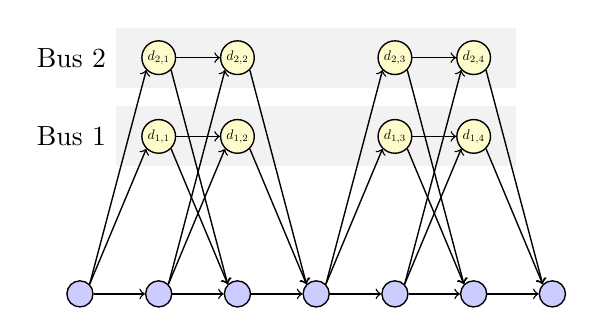
\begin{tikzpicture} 

		\node[rectangle, fill=gray!10, minimum width=2in, minimum height=.3in,label=left:Bus 2](bus2Box) at (3,3){};
		\node[rectangle, fill=gray!10, minimum width=2in, minimum height=.3in,label=left:Bus 1](bus1Box) at (3,2){};

		\node[circle, fill=blue!20, line width=0.5pt, draw=black, minimum size=0.1in](one) at (0,0){};
		\node[circle, fill=blue!20, line width=0.5pt, draw=black, minimum size=0.1in](two) at (1,0){}; 
		\node[circle, fill=blue!20, line width=0.5pt, draw=black, minimum size=0.1in](three) at (2,0){};
		\node[circle, fill=blue!20, line width=0.5pt, draw=black, minimum size=0.1in](four) at (3,0){};
		\node[circle, fill=blue!20, line width=0.5pt, draw=black, minimum size=0.1in](five) at (4,0){};
		\node[circle, fill=blue!20, line width=0.5pt, draw=black, minimum size=0.1in](six) at (5,0){};
		\node[circle, fill=blue!20, line width=0.5pt, draw=black, minimum size=0.1in](seven) at (6,0){};
		
		\node[circle, fill=yellow!20, line width=0.5pt, draw=black, minimum size=0.1in, inner sep=1pt](eight) at (1,2){\scalebox{0.5}{$d_{1,1}$}};
		\node[circle, fill=yellow!20, line width=0.5pt, draw=black, minimum size=0.1in, inner sep=1pt](nine) at (2,2){\scalebox{0.5}{$d_{1,2}$}};
		\node[circle, fill=yellow!20, line width=0.5pt, draw=black, minimum size=0.1in, inner sep=1pt](ten) at (4,2){\scalebox{0.5}{$d_{1,3}$}}; 
		\node[circle, fill=yellow!20, line width=0.5pt, draw=black, minimum size=0.1in, inner sep=1pt](eleven) at (5,2){\scalebox{0.5}{$d_{1,4}$}}; 

		\node[circle, fill=yellow!20, line width=0.5pt, draw=black, minimum size=0.1in, inner sep=1pt](twelve) at (1,3){\scalebox{0.5}{$d_{2,1}$}};
		\node[circle, fill=yellow!20, line width=0.5pt, draw=black, minimum size=0.1in, inner sep=1pt](thirteen) at (2,3){\scalebox{0.5}{$d_{2,2}$}};
		\node[circle, fill=yellow!20, line width=0.5pt, draw=black, minimum size=0.1in, inner sep=1pt](fourteen) at (4,3){\scalebox{0.5}{$d_{2,3}$}}; 
		\node[circle, fill=yellow!20, line width=0.5pt, draw=black, minimum size=0.1in, inner sep=1pt](fifteen) at (5,3){\scalebox{0.5}{$d_{2,4}$}}; 

		\draw [->, line width=0.5pt] (one.east) -- (two.west);
		\draw [->, line width=0.5pt] (two.east) -- (three.west);
		\draw [->, line width=0.5pt] (three.east) -- (four.west);
		\draw [->, line width=0.5pt] (four.east) -- (five.west);
		\draw [->, line width=0.5pt] (five.east) -- (six.west);
		\draw [->, line width=0.5pt] (six.east) -- (seven.west);

		\draw [->, line width=0.5pt] (one.north east) -- (eight.south west);
		\draw [->, line width=0.5pt] (two.north east) -- (nine.south west);
		\draw [->, line width=0.5pt] (four.north east) -- (ten.south west);
		\draw [->, line width=0.5pt] (five.north east) -- (eleven.south west);
		\draw [->, line width=0.5pt] (eight.south east) -- (three.north west);
		\draw [->, line width=0.5pt] (nine.south east) -- (four.north west);
		\draw [->, line width=0.5pt] (ten.south east) -- (six.north west);
		\draw [->, line width=0.5pt] (eleven.south east) -- (seven.north west);
		\draw [->, line width=0.5pt] (eight.east) -- (nine.west);
		\draw [->, line width=0.5pt] (ten.east) -- (eleven.west); 

		\draw [->, line width=0.5pt] (one.north east) -- (twelve.south west);
		\draw [->, line width=0.5pt] (two.north east) -- (thirteen.south west);
		\draw [->, line width=0.5pt] (four.north east) -- (fourteen.south west);
		\draw [->, line width=0.5pt] (five.north east) -- (fifteen.south west);
		\draw [->, line width=0.5pt] (twelve.south east) -- (three.north west);
		\draw [->, line width=0.5pt] (thirteen.south east) -- (four.north west);
		\draw [->, line width=0.5pt] (fourteen.south east) -- (six.north west);
		\draw [->, line width=0.5pt] (fifteen.south east) -- (seven.north west);
		\draw [->, line width=0.5pt] (twelve.east) -- (thirteen.west);
		\draw [->, line width=0.5pt] (fourteen.east) -- (fifteen.west); 

	\end{tikzpicture}
	\caption{SOC indicators}
	\label{fig:socDiagram}
\end{figure}
\par When charging, the change in SOC associated with the ith bus at the jth charge edge is denoted $g_{i,j}$. Again, note that j is \textit{not} indicative of a time interval, rather it gives the \textit{index} of the \textit{charge edge} in use as shown in figure \ref{fig:dSocDiagram}.
\begin{figure}
	\centering
	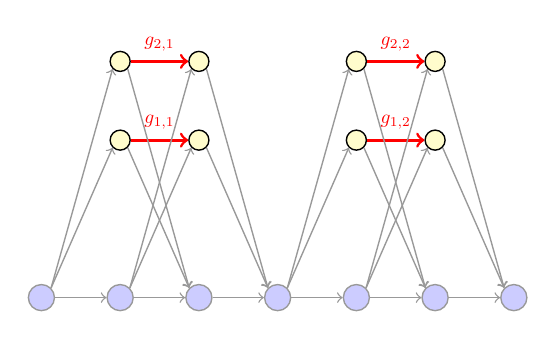
\begin{tikzpicture} 

		\node[circle, fill=blue!20, line width=0.5pt, draw=black!40, minimum size=0.1in](one) at (0,0){};
		\node[circle, fill=blue!20, line width=0.5pt, draw=black!40, minimum size=0.1in](two) at (1,0){}; 
		\node[circle, fill=blue!20, line width=0.5pt, draw=black!40, minimum size=0.1in](three) at (2,0){};
		\node[circle, fill=blue!20, line width=0.5pt, draw=black!40, minimum size=0.1in](four) at (3,0){};
		\node[circle, fill=blue!20, line width=0.5pt, draw=black!40, minimum size=0.1in](five) at (4,0){};
		\node[circle, fill=blue!20, line width=0.5pt, draw=black!40, minimum size=0.1in](six) at (5,0){};
		\node[circle, fill=blue!20, line width=0.5pt, draw=black!40, minimum size=0.1in](seven) at (6,0){};
		
		\node[circle, fill=yellow!20, line width=0.5pt, draw=black, minimum size=0.1in, inner sep=1pt](eight) at (1,2){};
		\node[circle, fill=yellow!20, line width=0.5pt, draw=black, minimum size=0.1in, inner sep=1pt](nine) at (2,2){};
		\node[circle, fill=yellow!20, line width=0.5pt, draw=black, minimum size=0.1in, inner sep=1pt](ten) at (4,2){};
		\node[circle, fill=yellow!20, line width=0.5pt, draw=black, minimum size=0.1in, inner sep=1pt](eleven) at (5,2){};

		\node[circle, fill=yellow!20, line width=0.5pt, draw=black, minimum size=0.1in, inner sep=1pt](twelve) at (1,3){};
		\node[circle, fill=yellow!20, line width=0.5pt, draw=black, minimum size=0.1in, inner sep=1pt](thirteen) at (2,3){};
		\node[circle, fill=yellow!20, line width=0.5pt, draw=black, minimum size=0.1in, inner sep=1pt](fourteen) at (4,3){};
		\node[circle, fill=yellow!20, line width=0.5pt, draw=black, minimum size=0.1in, inner sep=1pt](fifteen) at (5,3){};

		\draw [->, line width=0.5pt, color=black!40] (one.east) -- (two.west);
		\draw [->, line width=0.5pt, color=black!40] (two.east) -- (three.west);
		\draw [->, line width=0.5pt, color=black!40] (three.east) -- (four.west);
		\draw [->, line width=0.5pt, color=black!40] (four.east) -- (five.west);
		\draw [->, line width=0.5pt, color=black!40] (five.east) -- (six.west);
		\draw [->, line width=0.5pt, color=black!40] (six.east) -- (seven.west);

		\draw [->, line width=0.5pt, color=black!40] (one.north east) -- (eight.south west);
		\draw [->, line width=0.5pt, color=black!40] (two.north east) -- (nine.south west);
		\draw [->, line width=0.5pt, color=black!40] (four.north east) -- (ten.south west);
		\draw [->, line width=0.5pt, color=black!40] (five.north east) -- (eleven.south west);
		\draw [->, line width=0.5pt, color=black!40] (eight.south east) -- (three.north west);
		\draw [->, line width=0.5pt, color=black!40] (nine.south east) -- (four.north west);
		\draw [->, line width=0.5pt, color=black!40] (ten.south east) -- (six.north west);
		\draw [->, line width=0.5pt, color=black!40] (eleven.south east) -- (seven.north west);
		\draw [->, line width=1pt, color=red] (eight.east) -- node[above]{\scalebox{0.7}{$g_{1,1}$}}(nine.west);
		\draw [->, line width=1pt, color=red] (ten.east) -- node[above]{\scalebox{0.7}{$g_{1,2}$}}(eleven.west); 

		\draw [->, line width=0.5pt, color=black!40] (one.north east) -- (twelve.south west);
		\draw [->, line width=0.5pt, color=black!40] (two.north east) -- (thirteen.south west);
		\draw [->, line width=0.5pt, color=black!40] (four.north east) -- (fourteen.south west);
		\draw [->, line width=0.5pt, color=black!40] (five.north east) -- (fifteen.south west);
		\draw [->, line width=0.5pt, color=black!40] (twelve.south east) -- (three.north west);
		\draw [->, line width=0.5pt, color=black!40] (thirteen.south east) -- (four.north west);
		\draw [->, line width=0.5pt, color=black!40] (fourteen.south east) -- (six.north west);
		\draw [->, line width=0.5pt, color=black!40] (fifteen.south east) -- (seven.north west);
		\draw [->, line width=1pt, color=red] (twelve.east) -- node[above]{\scalebox{0.7}{$g_{2,1}$}}(thirteen.west);
		\draw [->, line width=1pt, color=red] (fourteen.east) -- node[above]{\scalebox{0.7}{$g_{2,2}$}}(fifteen.west); 

	\end{tikzpicture}
	\caption{Depiction of which edges increase SOC for the single rate case}
	\label{fig:dSocDiagram}
\end{figure}
\par An additional contribution this paper gives is the addition of multi-rate charging.  This adapts the basic methodology to incorporate additional charge edges and $g_{i,j}$ variables.  Under this methodology, the graph given in figure \ref{fig:groups} would be modified to reflect figure \ref{fig:multiRateChargeEdges}, where $g_{i,j,k}$ represents the ith bus at charge instance j and charge rate k.
\begin{figure}
	\centering
	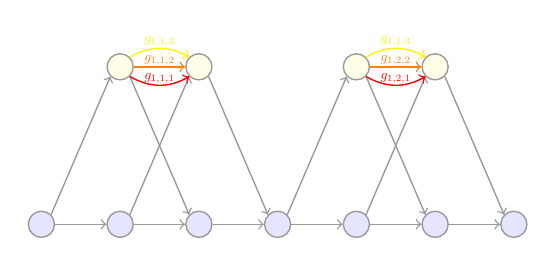
\begin{tikzpicture}[->, line width=0.5pt]
		\node[circle, fill=blue!10, draw=black!40,line width=0.5pt, minimum size=0.1in](one) at (0,0){};
		\node[circle, fill=blue!10, draw=black!40,line width=0.5pt, minimum size=0.1in](two) at (1,0){}; 
		\node[circle, fill=blue!10, draw=black!40,line width=0.5pt, minimum size=0.1in](three) at (2,0){};
		\node[circle, fill=blue!10, draw=black!40,line width=0.5pt, minimum size=0.1in](four) at (3,0){};
		\node[circle, fill=blue!10, draw=black!40,line width=0.5pt, minimum size=0.1in](five) at (4,0){};
		\node[circle, fill=blue!10, draw=black!40,line width=0.5pt, minimum size=0.1in](six) at (5,0){};
		\node[circle, fill=blue!10, draw=black!40,line width=0.5pt, minimum size=0.1in](seven) at (6,0){};
		\node[circle, fill=yellow!10, draw=black!40,line width=0.5pt, minimum size=0.1in](eight) at (1,2){};
		\node[circle, fill=yellow!10, draw=black!40,line width=0.5pt, minimum size=0.1in](nine) at (2,2){};
		\node[circle, fill=yellow!10, draw=black!40,line width=0.5pt, minimum size=0.1in](ten) at (4,2){}; 
		\node[circle, fill=yellow!10, draw=black!40,line width=0.5pt, minimum size=0.1in](eleven) at (5,2){}; 
		\draw [line width=0.5pt,color=black!40] (one.east) -- (two.west);
		\draw [line width=0.5pt,color=black!40] (two.east) -- (three.west);
		\draw [line width=0.5pt,color=black!40] (three.east) -- (four.west);
		\draw [line width=0.5pt,color=black!40] (four.east) -- (five.west);
		\draw [line width=0.5pt,color=black!40] (five.east) -- (six.west);
		\draw [line width=0.5pt,color=black!40] (six.east) -- (seven.west);
		\draw [line width=0.5pt,color=black!40] (one.north east) -- (eight.south west);
		\draw [line width=0.5pt,color=black!40] (two.north east) -- (nine.south west);
		\draw [line width=0.5pt,color=black!40] (four.north east) -- (ten.south west);
		\draw [line width=0.5pt,color=black!40] (five.north east) -- (eleven.south west);
		\draw [line width=0.5pt,color=black!40] (eight.south east) -- (three.north west);
		\draw [line width=0.5pt,color=black!40] (nine.south east) -- (four.north west);
		\draw [line width=0.5pt,color=black!40] (ten.south east) -- (six.north west);
		\draw [line width=0.5pt,color=black!40] (eleven.south east) -- (seven.north west);

		\draw [color=yellow,-,line width=0.5pt] (eight.north east) edge[->,bend left]node[above=-3pt]{\scalebox{0.5}{$g_{1,1,3}$}}(nine.north west);
		\draw [color=orange,line width=0.5pt] (eight.east) -- node[above=-3pt]{\scalebox{0.5}{$g_{1,1,2}$}}(nine.west);
		\draw [color=red,-,line width=0.5pt] (eight.south east) edge[->, bend right]node[above=-3pt]{\scalebox{0.5}{$g_{1,1,1}$}}(nine.south west);

		\draw [color=yellow,-, line width=0.5pt] (ten.north east) edge[->, bend left]node[above=-3pt]{\scalebox{0.5}{$g_{1,1,3}$}}(eleven.north west);
		\draw [color=orange,line width=0.5pt] (ten.east) -- node[above=-3pt]{\scalebox{0.5}{$g_{1,2,2}$}}(eleven.west); 
		\draw [color=red,-, line width=0.5pt] (ten.south east) edge[->, bend right]node[above=-3pt]{\scalebox{0.5}{$g_{1,2,1}$}}(eleven.south west);
	\end{tikzpicture}
	\caption{Multi-Rate Charging}
	\label{fig:multiRateChargeEdges}
\end{figure}
\par To model the effect of charging on a battery state of charge, we adopt the Constant Current Constant Voltage (CCCV) model as derived in \cite{whitaker_network_2021} which gives
\begin{align}
	s_{k+1} = \bar{a}_ls_k - \bar{b}_lM 
\end{align}
Where $s_k$ is the charge of a battery at time $k$, $\bar{a}_l$ is a charge rate dependent, experimentally determined value, $\bar{b_l} = \bar{a_l} - 1$, and $M$ is the maximum capacity of the battery in kWh.  
\par Recall how $g$ represented the change in state of charge of the battery in kWh.  This allows us to express $s_{k+1}$ in terms of 
\begin{align}
	s_{k+1} = s_k + g_{\pi_g(m,k,l)}
\end{align}
where $\pi_g(m,k,l)$ represents the index of $g$ for bus $m$ at time index $k$ for charge rate $l$.  These two equations imply that
\begin{equation}
\begin{aligned}
	s_k + g_{\pi_g(m,k,l)} &= \bar{a}_ls_k - \bar{b}_lM \\
\Rightarrow g_{\pi_g(m,k,l)} &=  \bar{a}_ls_k - s_k - \bar{b}_lM \\
\Rightarrow g_{\pi_g(m,k,l)} &=  s_k(\bar{a}_l - 1) - \bar{b}_lM.
\end{aligned}
\end{equation}
But the state of charges for bus $m$ are given in terms of $d_{i,j}$.  If we let $d_{i,j} = \pi_d(i,k,l)$, then the final expression for $g$ becomes
\begin{align}\label{eqn:g}
	g_{\pi_g(m,k,l)} = d_{\pi_d(m,k,l)}(\bar{a}_l - 1) - \bar{b}_lM.
\end{align}
Note, \ref{eqn:g} is only valid when the bus is charging and must be tempered with additional constraints to account for the non-charging case.
\par To handle the two cases, we express the cases for charging (equation \ref{eqn:g} and non-charging ($g=0$) as  
\begin{equation}
\begin{aligned}
	g_{\pi_g(m,k,l)}  &= d_{\pi_d(m,k,l)}(\bar{a}_l - 1) - \bar{b}_lM \\
	g_{\pi_g(m,k,l)} &= 0.
\end{aligned}
\end{equation}
which also implies that
\begin{equation}\label{eqn:gTwoConst}
\begin{aligned}
	g_{\pi_g(m,k,l)}  &\le d_{\pi_d(m,k,l)}(\bar{a}_l - 1) - \bar{b}_lM \\
	g_{\pi_g(m,k,l)}  &\ge d_{\pi_d(m,k,l)}(\bar{a}_l - 1) - \bar{b}_lM \\
	g_{\pi_g(m,k,l)} &\le 0 \\
	g_{\pi_g(m,k,l)} &\ge 0.
\end{aligned}
\end{equation}
Next, let $x_{\pi_x(m,k,l)}$ be the index of the edge corresponding to $g_{\pi_g(m,k,l)}$.  A switch between the two constarints expressed in equation \ref{eqn:gTwoConst} can be constructed using the \textit{big M} technique.  This modifies equation \ref{eqn:gTwoConst} such that
\begin{equation}\label{eqn:gBigM}
	\begin{aligned}
		g_{\pi_g(m,k,l)}  &\le d_{\pi_d(m,k,l)}(\bar{a}_l - 1) - \bar{b}_lM - M(1 - x_{\pi_x(m,k,l)})\\
		g_{\pi_g(m,k,l)}  &\ge d_{\pi_d(m,k,l)}(\bar{a}_l - 1) - \bar{b}_lM \\
		g_{\pi_g(m,k,l)} &\le 0 + Mx_{\pi_x(m,k,l)})\\
		g_{\pi_g(m,k,l)} &\ge 0.  
	\end{aligned}
\end{equation}
Note that as expressed, when the charge edge is active (i.e. $x_{\pi_x(m,k,l)} = 1$), then 
\begin{equation}
	\begin{aligned}
		\color{blue}{g_{\pi_g(m,k,l)}}  &\color{blue}{\le d_{\pi_d(m,k,l)}(\bar{a}_l - 1) - \bar{b}_lM} \\
		\color{blue}{g_{\pi_g(m,k,l)}}  &\color{blue}{\ge d_{\pi_d(m,k,l)}(\bar{a}_l - 1) - \bar{b}_lM} \\
		\color{red}{g_{\pi_g(m,k,l)}} & \color{red}{\le M} \\
		\color{red}{g_{\pi_g(m,k,l)}} & \color{red}{\ge 0}.  
	\end{aligned}
\end{equation}
Bus as $g$ can never exceed the charge capacity of the battery, the bottom two constraints are inactive and $g$ is both less than or greater than equation \ref{eqn:g}, making it equal.  When the edge is inactive, or $x_{\pi_x(m,k,l)} = 0$, equation \ref{eqn:gBigM} becomes
\begin{equation}
	\begin{aligned}
		\color{red}{g_{\pi_g(m,k,l)}}  &\color{red}{\le d_{\pi_d(m,k,l)}(\bar{a}_l - 1) - \bar{b}_lM - M} \\
		\color{red}{g_{\pi_g(m,k,l)}}  &\color{red}{\ge d_{\pi_d(m,k,l)}(\bar{a}_l - 1) - \bar{b}_lM} \\
		\color{blue}{g_{\pi_g(m,k,l)}} &\color{blue}{\le 0} \\
		\color{blue}{g_{\pi_g(m,k,l)}} &\color{blue}{\ge 0}.  
	\end{aligned}
\end{equation}
where the top two constraints become inactive and $g$ is both less than and greater than 0, making it equal.
Hence, these constraints can be expressed in linear form as
\begin{equation}\label{eqn:chargeConstraints}
	\begin{aligned} 
		-g_{m,k,l} + d_{m,k,l}(\bar{a}_l - 1) + x_{m,k,l} &\le M(\bar{b}_l + 1) \\
		 g_{m,k,l} - d_{m,k,l}(\bar{a}_l - 1)  &\le  - \bar{b}_lM \\
		 g_{m,k,l} - Mx_{m,k,l} &\le 0 \\
		-g_{m,k,l} &\le 0.  
	\end{aligned}
\end{equation}
\par The constraints for state of charge are circumstantially dependent. Each $d_{m,k,l}$ must be defined by a set of constraints which are defined by either initial conditions, previous graphs, route discharge, or $g_{m,k,l}$ variables.
\par Initial conditions and previous graphs are straight forward.  Initial conditions are given as an equality constraint.  For example, if $d_0$ was initialized to 80 kWh, the constraint would be $d_0 = 80$.  To initialize to the value of a previous graph, use an equality constraint.  
\par Suppose we modeled early morning and day-time operations and had two corresponding graphs. The final node of graph one would be equivalent to the first node of graph two in the temporal sense and the corresponding $d_{m,l,k}$ values would also be equated as $d_{\text{Graph 1}} - d_{\text{Graph 2}} = 0$.
\par $d_{m,l,k}$ values corresponding to available charge times are expressed as a sum of $g_{m,k,l}$ values given in equation \ref{eqn:chargeConstraints} such that
\begin{align*}
	d_{m,k + 1} = d_{m,k} + \sum_l{g_{m,k,l}}
\end{align*}
or as given in linear form,
\begin{align}
	d_{m,k+1} - d_{m,k} - \sum_l{g_{m,k,l}} = 0.
\end{align}
\par The final case deals with battery discharge over a route.  As seen in figure \ref{fig:delta}, discharge values, also refered to as $\delta$ represent the power expenditure overa route.  This expenditure is modeled as a withdrawel from the resevour in a battery and was calibrated from data received from the Utah Transit Authority.  In figure \ref{fig:delta}, the SOC constraints corresponding to $\delta_1$ would be as follow:
\begin{align*}
	d_{1,3} = d_{1,2} - \delta_1
\end{align*}
or in linear form,
\begin{align}
	d_{1,2} - d_{1,3} = \delta_1.
\end{align}
\begin{figure}
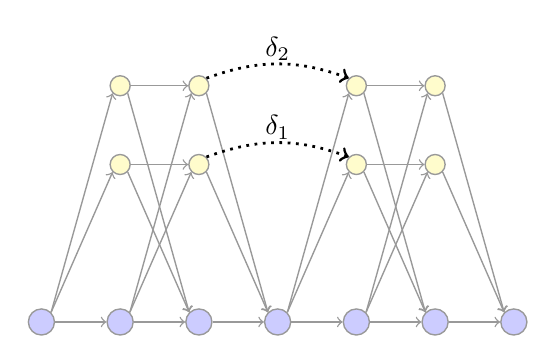
\begin{tikzpicture}
	\node[circle, fill=blue!20, line width=0.5pt, draw=black!40, minimum size=0.1in](one) at (0,0){};
	\node[circle, fill=blue!20, line width=0.5pt, draw=black!40, minimum size=0.1in](two) at (1,0){}; 
	\node[circle, fill=blue!20, line width=0.5pt, draw=black!40, minimum size=0.1in](three) at (2,0){};
	\node[circle, fill=blue!20, line width=0.5pt, draw=black!40, minimum size=0.1in](four) at (3,0){};
	\node[circle, fill=blue!20, line width=0.5pt, draw=black!40, minimum size=0.1in](five) at (4,0){};
	\node[circle, fill=blue!20, line width=0.5pt, draw=black!40, minimum size=0.1in](six) at (5,0){};
	\node[circle, fill=blue!20, line width=0.5pt, draw=black!40, minimum size=0.1in](seven) at (6,0){};
	
	\node[circle, fill=yellow!20, line width=0.5pt, draw=black!40, minimum size=0.1in, inner sep=1pt](eight) at (1,2){};
	\node[circle, fill=yellow!20, line width=0.5pt, draw=black!40, minimum size=0.1in, inner sep=1pt](nine) at (2,2){};
	\node[circle, fill=yellow!20, line width=0.5pt, draw=black!40, minimum size=0.1in, inner sep=1pt](ten) at (4,2){};
	\node[circle, fill=yellow!20, line width=0.5pt, draw=black!40, minimum size=0.1in, inner sep=1pt](eleven) at (5,2){};

	\node[circle, fill=yellow!20, line width=0.5pt, draw=black!40, minimum size=0.1in, inner sep=1pt](twelve) at (1,3){};
	\node[circle, fill=yellow!20, line width=0.5pt, draw=black!40, minimum size=0.1in, inner sep=1pt](thirteen) at (2,3){};
	\node[circle, fill=yellow!20, line width=0.5pt, draw=black!40, minimum size=0.1in, inner sep=1pt](fourteen) at (4,3){};
	\node[circle, fill=yellow!20, line width=0.5pt, draw=black!40, minimum size=0.1in, inner sep=1pt](fifteen) at (5,3){};

	\draw [->, line width=0.5pt, color=black!40] (one.east) -- (two.west);
	\draw [->, line width=0.5pt, color=black!40] (two.east) -- (three.west);
	\draw [->, line width=0.5pt, color=black!40] (three.east) -- (four.west);
	\draw [->, line width=0.5pt, color=black!40] (four.east) -- (five.west);
	\draw [->, line width=0.5pt, color=black!40] (five.east) -- (six.west);
	\draw [->, line width=0.5pt, color=black!40] (six.east) -- (seven.west);

	\draw [->, line width=0.5pt, color=black!40] (one.north east) -- (eight.south west);
	\draw [->, line width=0.5pt, color=black!40] (two.north east) -- (nine.south west);
	\draw [->, line width=0.5pt, color=black!40] (four.north east) -- (ten.south west);
	\draw [->, line width=0.5pt, color=black!40] (five.north east) -- (eleven.south west);
	\draw [->, line width=0.5pt, color=black!40] (eight.south east) -- (three.north west);
	\draw [->, line width=0.5pt, color=black!40] (nine.south east) -- (four.north west);
	\draw [->, line width=0.5pt, color=black!40] (ten.south east) -- (six.north west);
	\draw [->, line width=0.5pt, color=black!40] (eleven.south east) -- (seven.north west);
	\draw [->, line width=0.5pt, color=black!40] (eight.east) -- (nine.west);
	\draw [->, line width=0.5pt, color=black!40] (ten.east) -- (eleven.west); 

	\draw [->, line width=0.5pt, color=black!40] (one.north east) -- (twelve.south west);
	\draw [->, line width=0.5pt, color=black!40] (two.north east) -- (thirteen.south west);
	\draw [->, line width=0.5pt, color=black!40] (four.north east) -- (fourteen.south west);
	\draw [->, line width=0.5pt, color=black!40] (five.north east) -- (fifteen.south west);
	\draw [->, line width=0.5pt, color=black!40] (twelve.south east) -- (three.north west);
	\draw [->, line width=0.5pt, color=black!40] (thirteen.south east) -- (four.north west);
	\draw [->, line width=0.5pt, color=black!40] (fourteen.south east) -- (six.north west);
	\draw [->, line width=0.5pt, color=black!40] (fifteen.south east) -- (seven.north west);
	\draw [->, line width=0.5pt, color=black!40] (twelve.east) -- (thirteen.west);
	\draw [->, line width=0.5pt, color=black!40] (fourteen.east) -- (fifteen.west); 
	\draw [dotted, color=black,-,line width=1pt] (nine.north east) edge[->,bend left=20pt]node[above=-2.5pt]{\scalebox{1}{$\delta_1$}}(ten.north west); 
	\draw [dotted, color=black,-,line width=1pt] (thirteen.north east) edge[->,bend left=20pt]node[above=-2.5pt]{\scalebox{1}{$\delta_2$}}(fourteen.north west); 
\end{tikzpicture}
	\caption{$\delta$ values for routes}
	\label{fig:delta}
\end{figure} 

\section{Fiscal Rate Schedule}
One objective of this work is to minimize the fiscal cost associated with power use and uses the Rocky Mountain Power schedule 8 billing rates. This billing schedule includes an on-peak power charge, facilities charge, and both on and off peak energy charges.
\par The facilities charge is computed by calculating the average power over a 15 minute period.  The facilities charge is based on the maximum average value over the course of the month.  This section of the bill charges \$4.81 per kW. The On-Peak Power Charge is similarly calculated but only includes average values from designated on-peak hours.  Rocky Mountain Power charges \$15.73 per kW for this value.
\par the facilities power can be formulated as a linear set of constraints that include power used at each timestep for charging buses and external loads.  This can be expressed as 
\begin{align*}
	c_i = \sum_j{g_{i,j}} + p_i
\end{align*}
Where $c_i$ represnets the 
\par  The energy charges are billed per kWh and charge for each unit of energy used.  There are two rates: 5.8282\textcent for energy consumed during on-peak hours, and 2.6316\textcent for off-peak hours.
general introduction with details for demand and consumption charge and how these relate to the end-of-the-month billing.

    a. external loads (contribution)
    b. consumption charge
        i. total energy in Kwh
	ii. on-peak vs off-peak
	iii. constraints for consumption charge
    c. demand charge
        i. average power in 15 minute window
	ii. on-peak vs facilities 
	iii. constraints for on-peak and facilities charges
    d. total cost breakdown
        i. Show how Rocky Mountain Power uses these and what the cost weighting is.

\section{Bus Fleet Operations}
Overview of bus operations during the day vs the night
    a. night environment
        i. one charger per bus
        ii. slow chargers
        iii. single rate chargers
        iv. buses always available
    b. day environment
        i. limited number of chargers
        ii. fast/variable rates
        iii. limited charging availability
    c. multiple graphs to incorporate day vs night charging
        i. show picture to illustrate this
	ii. show SOC constraints to implement these relationships



